\section{Experimental Design}
\label{sec:experiment-design}

Two experiments were conducted to evaluate the performance of a selected set of \ac{llms} in generating questions. The first experiment primarily focused on the \textbf{RQ1}, which aimed to assess the content fidelity of the generated questions according to the \ac{llms} and the diverse source materials. The second experiment was designed to answer \textbf{RQ2}, which focused on analyzing the relationships between the \ac{llms}, given questions formats and given levels of Bloom's revised Taxonomy \cite{krathwohl_revision_2002}.

\begin{figure}[htbp]
    \centering
    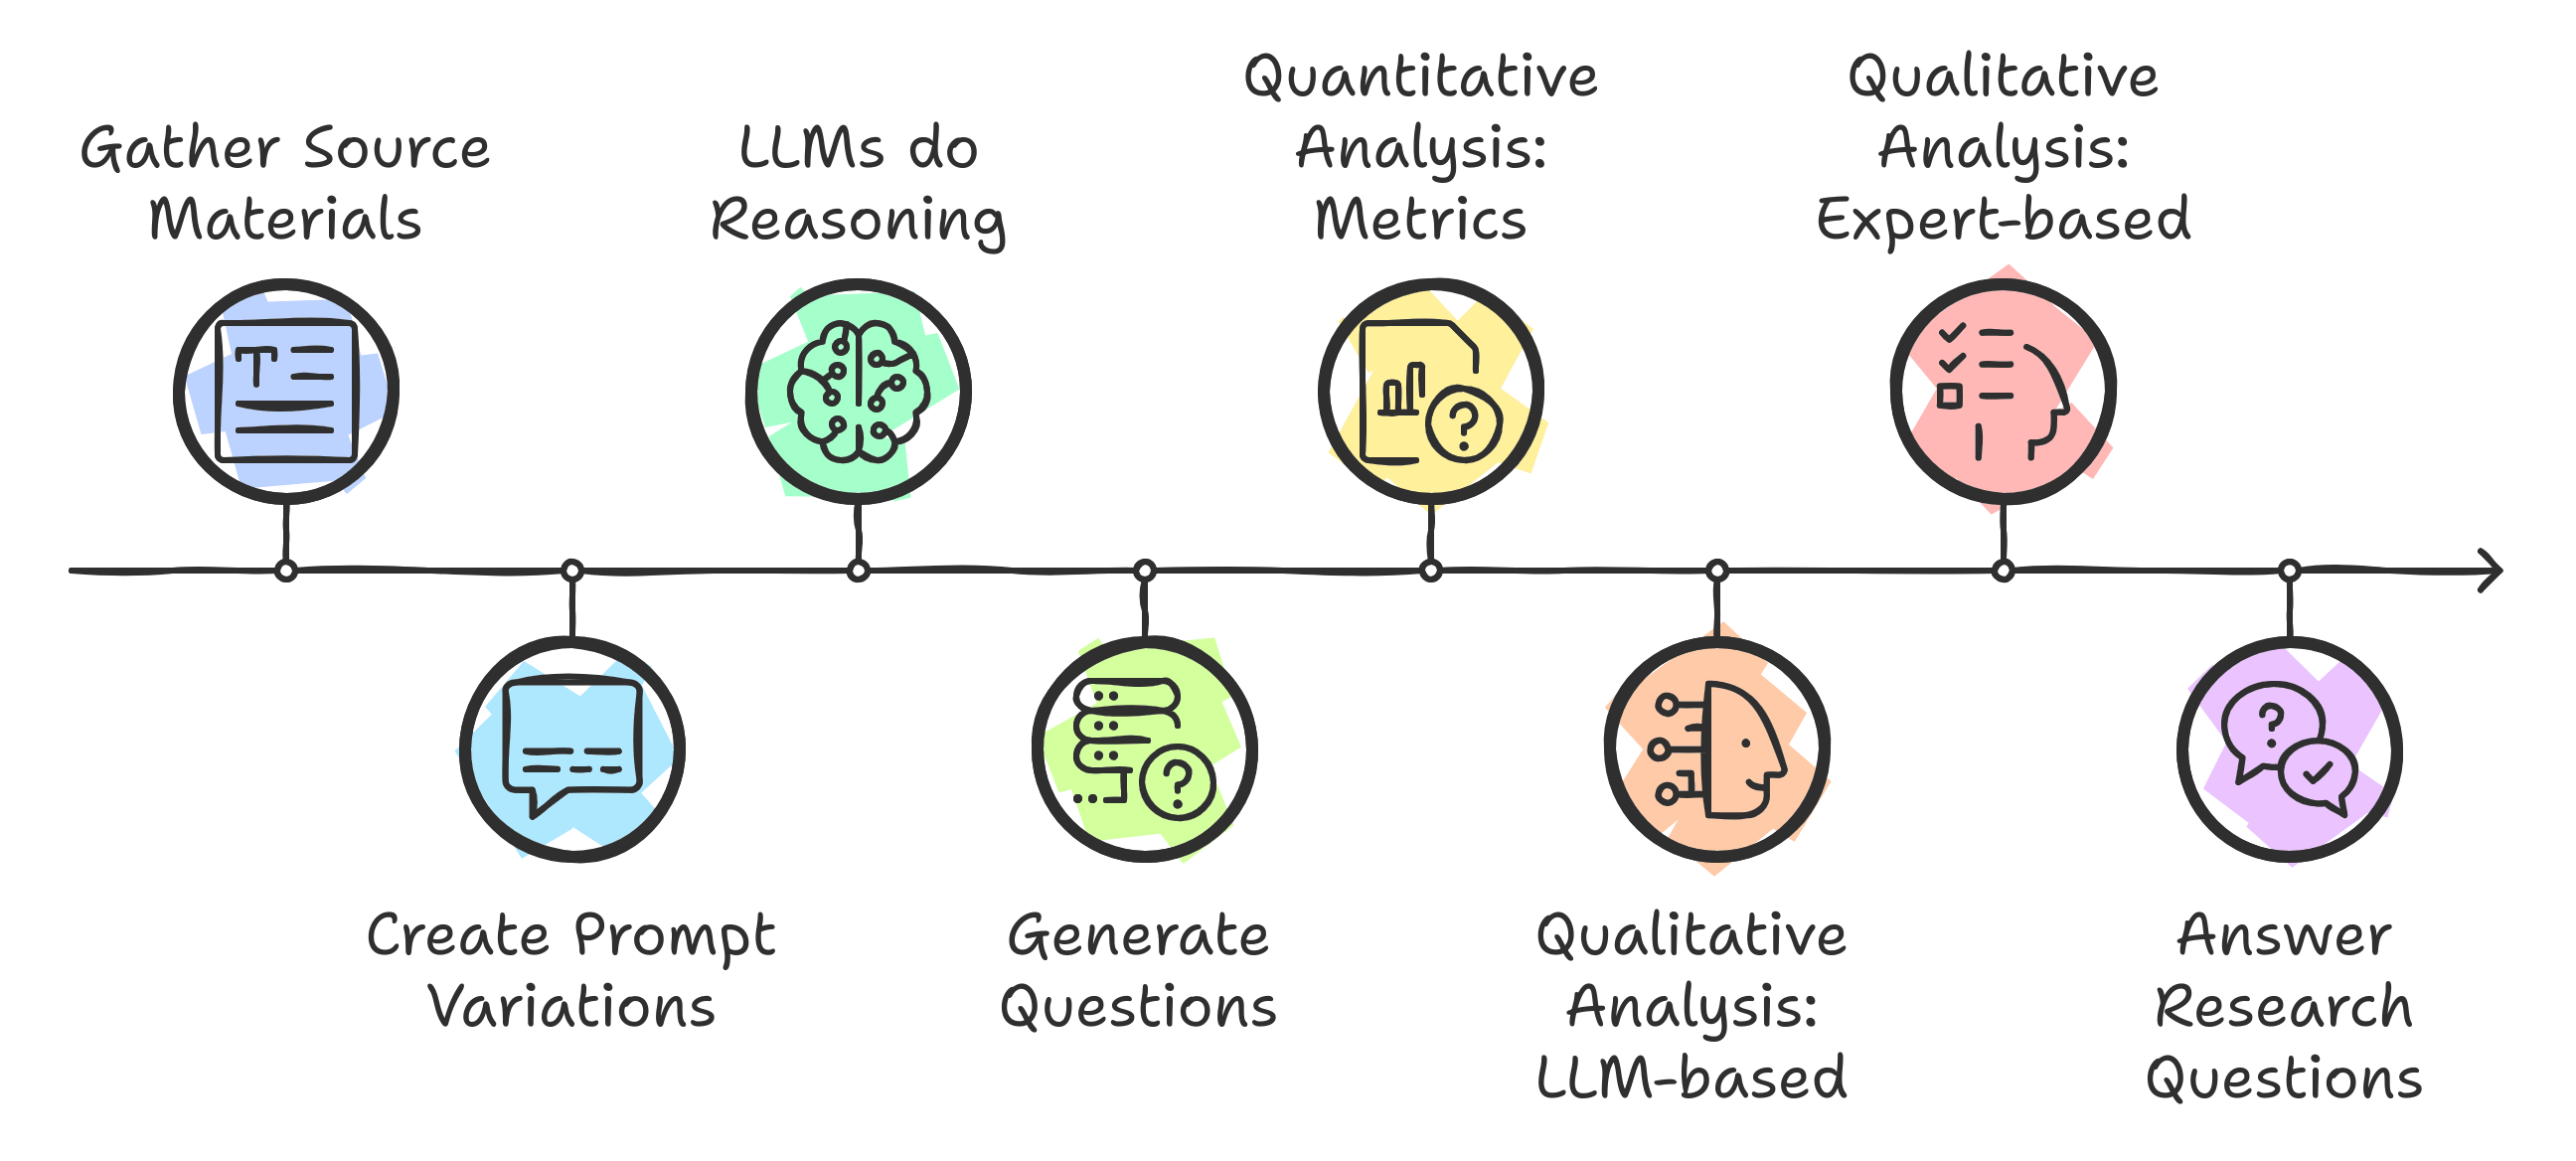
\includegraphics[width=\textwidth]{../extra/approach.png}
    \caption[Experimental Pipeline.]{Experimental Pipeline\footnotemark.}
    \label{fig:experiment-overview}
\end{figure}
\footnotetext{created with \url{https://www.napkin.ai/}, accessed 05/24/2025}
\vspace{-1em}
    
\subsection{Selection of Resources}
\label{sec:selection-resources}

To ensure the experiments were well-structured and relevant, a variety of resources were selected. This covers the source materials and the \ac{llms} used in the experiments for \ac{aqg}.

\object{Selection of Source Materials}
Focusing on the subject of the ISO-OSI model, the following materials, illustrated \bfhyperref{sec:source_materials}{here}, were diversely used to generate the experiments' questions:

\begin{itemize}
    \item \bfhyperref{sec:script-common}{Lecture Slides} \textbf{(extracted Part)}: Dealing with reference architectures, the ISO-OSI model is presented in detail. The slides are in German and were used for \ac{aqg} for the first experiment.
    \item \bfhyperref{sec:transcript}{Transcript} \textbf{(Lecture's Video Part)}: The transcript of the extracted slides is in German and was also used to generate questions for the first experiment.
    \item \bfhyperref{sec:tanenbaum}{Book's Excerpt} \textbf{(from \enquote{Computer Networks})} \cite{tanenbaum_computer_2013}: This book is in English and was used to generate questions for both experiments, with a detailed description of the ISO-OSI model, including all seven layers.
\end{itemize}

To properly challenge the \ac{llms} in their multilingual capabilities, each source material was kept in its original language: German for the lecture slides and its transcript, the book excerpt in English.

\pagebreak

\object{Selection of \ac{llms}} A total of four \ac{llms} were selected for both experiments, which belong to the current state-of-the-art in the field of \ac{llms} and are publicly available to certain degrees, and incorporate reasoning capabilities. The selected models are:
Anthropic Claude 3.7 Sonnet \cite{anthropic_claude_2025},
    DeepSeek R1 \cite{deepseek-ai_deepseek-r1_2025},
    Google Gemini 2.5 Flash \cite{kavukcuoglu_gemini_2025}, and
    OpenAI o3 \cite{openai_openai_2025-1}.

\vspace{1em}

o3 and Claude 3.7 Sonnet were accessed through their Python APIs\footnote{\label{fn:openai-api}\url{https://github.com/openai/openai-python}, accessed 05/09/2025}\footnote{\label{fn:anthropic-api}\url{https://github.com/anthropics/anthropic-sdk-python}, accessed 05/09/2025}, incurring costs per usage. This access method was necessary as the chosen models were not available to the required extent through other means. In contrast, Gemini 2.5 Flash was utilized via Google's Python API\footnote{\label{fn:google-api}\url{https://github.com/googleapis/python-genai}, accessed 05/09/2025}, which offers a free usage tier. To manage costs while maintaining a robust set of \ac{llms}, DeepSeek R1, a comparatively less expensive yet highly capable \ac{llm}, was accessed free of charge via its website\footnote{\label{fn:deepseek}\url{https://chat.deepseek.com/}, accessed 05/09/2025}.

\subsection{Methodological Approach}
\label{sec:methodological-approach}

The method employed for the two experiments is outlined here. It details the specific procedures for generating questions, including the variations in source materials, \ac{llm} prompting strategies, and the targeted number of questions for each experimental condition.

% \object{Experiment 1a: Content Fidelity} The presented 4 source materials were used to generate questions. The 4 state-of-the-art \ac{llms} were used, each model was prompted with the 4 input types each via a common prompt and a complex prompt. 
% \newtodo{Think about splitting the inputs into 7 groups, related to the 7 ISO-OSI layers.}
% This would result a final set of questions: 4 materials / or 28 if thinking about the 7 layers, 4 \ac{llms}, 5 questions for each prompt, 2 prompts, $4\cdot 4\cdot 5\cdot 2=160$

\object{Experiment 1a: Content Fidelity} For the first experiment, questions were generated using the three selected source materials to compare the questions' quality. All four state-of-the-art \ac{llms} were employed. Each model was prompted using both a simple and a complex prompt. To prevent context spillover and ensure focused questioning, one question was generated per prompt for each of the seven layers of the ISO-OSI model, with the context for each layer being introduced in each distinct run. This methodology resulted in a total of \begin{align}4 \text{ \ac{llms}} \times 3 \text{ input sources} \times 7 \text{ layers} \times 1 \sfrac{\text{ question}}{\text{prompt}} \times 2 \text{ prompts} = 168 \text{ questions.}\end{align}

% \object{Experiment 1b: Error Propagation} A second run is to be done. The same experimental setup as in Experiment 1a was used, but the source materials were manipulated. I have to choose a certain layer of the ISO-OSI model and manipulate the source materials for this layer. So there is 1 layer only, and 3 source materials (the system knowledge only is not used). 4 \ac{llms} used again, 5 questions per prompt, 1 prompt (the complex and better one). This results in a final set of questions: $1\cdot 3\cdot 4\cdot 5\cdot 1=60$.

\object{Experiment 1b: Error Propagation} A subsequent run focused on error propagation. The four \ac{llms} were again utilized with both simple and complex prompts. For this experiment, a single input source, specifically the lecture script -- chosen for its concise and precise contextual information -- was used. Each of the seven layers of the ISO-OSI model within this source material was intentionally manipulated to introduce errors, as to be seen \bfhyperref{sec:script-manipulated}{here}. Seven questions were generated per prompt, one for each manipulated layer and run. This resulted in a total of \begin{align}4 \text{ \ac{llms}} \times 1 \text{ input source} \times 7 \text{ layers} \times 1 \sfrac{\text{ question}}{\text{prompt}} \times 2 \text{ prompts} = 56 \text{ questions.}\end{align}

\pagebreak

\object{Experiment 2: Question Formats and Bloom's Taxonomy} The second experiment focused on the generation of varied question formats and their alignment with Bloom's revised Taxonomy. Contextual information for this experiment was derived from a single, pre-selected layer of the ISO-OSI model, utilizing the detailed content from \bfhyperref{lst:tanenbaum_layer2}{Layer 2} within the excerpt from \cite{tanenbaum_computer_2013}. The four selected \ac{llms} were employed in three distinct runs, each designed to explore different prompting parameters related to question type and cognitive complexity:

\begin{enumerate}
    \item \textit{Question Type Specification}: Prompts specified only the desired question types (Multiple-Choice and Open-Ended). For the chosen layer, each \ac{llm} was tasked six times to generate a question without mentioning a certain Bloom level for each of the two question types, resulting in \begin{align}4 \text{ \ac{llms}} \times 2 \text{ question types} \times 1 \sfrac{\text{ question}}{\text{run}}\times 6 \text{ runs} = 48 \text{ questions.}\end{align}
    \item \textit{Cognitive Level Specification}: Prompts specified only the target cognitive levels according to Bloom's Taxonomy. For the chosen layer, each \ac{llm} generated one question for six runs to get a question for each of the Bloom levels. In total, these are  \begin{align}4 \text{ \ac{llms}} \times 1 \sfrac{\text{ question}}{\text{level}} \times 6 \text{ Bloom levels} = 24 \text{ questions.}\end{align}
    \item \textit{Combined Specification}: Prompts specified both the question types (Multiple-Choice and Open-Ended) and the cognitive levels. Similar to the first run, this resulted in \begin{align}4 \text{ \ac{llms}} \times 2 \text{ question types} \times 1 \sfrac{\text{ question}}{\text{level}} \times 6 \text{ Bloom levels} = 48 \text{ questions.}\end{align}
\end{enumerate}

\object{Data Collection} The data was primarily collected using the \ac{llms} via their APIs, excepting DeepSeek being prompted on the website. The other 3 models were prompted automatically via Python to generate questions based on the given source materials. The generated questions were stored in a directory structure, particularly based on the experiment, the \ac{llm} and the source material. The question files for each prompt were stored in distinct \textit{.txt} files.

\object{Evaluation Plan} The evaluation of the generated questions will be conducted in two phases, corresponding to the two main experiments. Each phase employs a multi-modal assessment combining automated metrics, LLM-based evaluation, and expert human annotation to ensure comprehensive quality assessment.
\begin{itemize}
    \item \textbf{Experiment 1 (Content Fidelity and Error Propagation):}
    \begin{itemize}
        \item \textit{Quantitative Analysis:} In this stage, the \textit{Semantic Similarity} between generated questions and source materials will be assessed using cosine similarity on generated text embedding vectors. This can be done since a sentence transformer is used, which offer comparable sentence embeddings \cite{reimers_sentence-bert_2019}. Metrics such as \textit{\ac{bleurt}} and \textit{\ac{rquge}} were not employed since, on the one hand, the structure of the source material and the question differ too much, and on the other hand, gold standard answers are not available for comparison.

        \pagebreak
        
        Moreover, other metrics such as Perplexity are less suitable for this task, as \enquote{the output value is based heavily on what the text and the model was trained on. This means that perplexity scores are not comparable between models or datasets}, as stated on HuggingFace\footnote{\url{https://huggingface.co/spaces/evaluate-metric/perplexity}}. Instead, to properly analyze the content fidelity on a quantitative level, the \textit{Content Adherence} will be assessed by prompting an \ac{llm}. By this, the generated questions can be evaluated against the source material by returning a value between 0 and 1. Regarding \cite{nguyen_reference-based_2024}, which used an \ac{llm} to extensively evaluate generated questions which are based on context, the authors did not cover the content adherence. This offers a new perspective on the evaluation of generated questions, especially in the context of \ac{aqg}.

        \item \textit{Qualitative Analysis:} An \ac{llm} will serve as an evaluator with multiple runs to ensure validity. Besides, expert evaluations are conducted on a sampled question subset using the same concise rubric. Inter-annotator agreement between the \ac{llm} and human experts (via Cohen's Kappa) will be measured to validate the reliability of automated evaluation. Since Experiment 1b examines the adherence to manipulated input texts, the \textit{Correctness} will be specifically assessed for each of the two experimental runs, as quantitative metrics solely may not capture the correctness of the generated questions. The evaluation adopts the rubric structure from \cite{mi_comparative_2024}, maintaining a maximum score of 50 points per question. However, the \textit{Bloom's Level} criterion is replaced with \textit{Correctness} to address the specific objectives of this experiment:

        \begin{table}[htbp]
           \centering
           \renewcommand{\arraystretch}{1.6}
           \caption{Experiment 1 Evaluation Criteria.}
           \label{tab:exp1_criteria}
           \begin{tabularx}{\textwidth}{|Z|A|Y|}
           \rowcolor{gray!15}
           \hline
           \textbf{Criterion} & \textbf{Description} & \textbf{Scoring} \\
           \hline
           \textbf{Relevance} & Is the question relevant to the topic of the source text? & 0-10p \\
           \hline
           \textbf{Clarity} & Is the question easy to understand \& the presentation logical and clear? & 0-10p \\
           \hline
           \textbf{Answerability} & Are students likely able to answer the question based on the provided material? & 0-10p \\
           \hline
           \textbf{Challenging} & Is the question challenging? Does it encourage students to think actively? & 0-10p \\
           \hline
           \multirow{2}{*}{\textbf{Correctness}} & \textbf{Original Source Material:} Is the question factually correct \& adhering to the source text? & \vspace{-1em}\begin{itemize} 
                \item Correct: 10p
                \item Partially correct: 5p
                \item Otherwise: 0p
            \end{itemize} \\
           \cline{2-3}
            & \textbf{Manipulated Source Material:} Does the question adhere to the manipulated input text content? & \vspace{-1em}\begin{itemize} 
                \item No Adherence: 10p
                \item Partially adheres: 5p
                \item Otherwise: 0p
            \end{itemize} \\
           \hline
           \end{tabularx}
         \end{table}
    \end{itemize}

    \pagebreak

    \item \textbf{Experiment 2 (Question Formats and Bloom's Taxonomy):}
    \begin{itemize}
        \item \textit{Qualitative Analysis:} As the primary focus of this experiment lies on qualitative assessment, any quantitative evaluation is discarded. An \ac{llm} will function as the primary evaluator, with expert evaluations conducted again on randomized samples. Inter-annotator agreement will be critical for validating the \ac{llm} as a reliable evaluator for this experiment as well. Both follow the rubric structure from the previously used \cite{mi_comparative_2024}, also maintaining a maximum score of 50 points per question. In this experiment, instead of evaluating the proposed \textit{Correctness}, the \text{Bloom's Level} is used again with specific refinements addressing Bloom's Taxonomy assessment:
        % \vspace{5em}
        % \pagebreak

        \begin{table}[htbp]
           \centering
           \renewcommand{\arraystretch}{1.6}
           \caption{Experiment 2 Evaluation Criteria.}
           \label{tab:exp2_criteria}
           \begin{tabularx}{\textwidth}{|Z|A|Y|}
           \rowcolor{gray!15}
           \hline
           \textbf{Criterion} & \textbf{Description} & \textbf{Scoring} \\
           \hline
           \textbf{Relevance} & Is the question relevant to the topic of the source text? & 0-10p \\
           \hline
           \textbf{Clarity} & Is the question easy to understand \& the presentation logical and clear? & 0-10p \\
           \hline
           \textbf{Answerability} & Are students likely able to answer the question based on their knowledge level? & 0-10p \\
           \hline
           \textbf{Challenging} & Is the question challenging? Does it encourage students to think actively? & 0-10p \\
           \hline
           \multirow{2}{*}{\textbf{Bloom's Level}} & \textbf{When Bloom level is specified:} Does the question adhere to the given Bloom level? & \vspace{-1em} \begin{itemize}
                \item Correct: 10p
                \item Off by one: 5p
                \item Otherwise: 0p
            \end{itemize} \\
           \cline{2-3}
            & \textbf{When no Bloom level is specified:} Which Bloom level does the question demonstrate? & \vspace{-1em} \begin{itemize}
                \item Creating: 10p
                \item Evaluating: 8.5p
                \item Analyzing: 7p
                \item Applying: 4.5p
                \item Understanding: 3p
                \item Remembering 1.5p
            \end{itemize} \\
           \hline
           \end{tabularx}
         \end{table}
    \end{itemize}
\end{itemize}

Since both the human and the \ac{llm}-based evaluation shall be conducted as blind tests, the evaluators also will not be aware of the desired Bloom level for each question. This ensures an unbiased assessment, resulting that the evaluators shall return solely the Bloom level they perceive for each question. Based on this, the scoring for \textit{Bloom's Level} will be conducted automatically based on the given scoring guideline in Table \bfref{tab:exp2_criteria}.

The details about the \bfhyperref{sec:implementation-and-execution}{Implementation and Execution} for this experimental setup will be presented below. The results and discussion of these evaluations will be presented in Section \bfref{sec:evaluation}.